\chapter{Methods}

\section{Literature Review}
\subsection{Earlier Work}
In recent years, researchers and analysts focused mainly on gray-scale face image. Others, focused and were built on pattern identification models, possessing information of the model while others used AdaBoost. \cite{ojala2002multiresolution} This was a superb classifier for the purpose of training. When Viola-Jones Detector came, which was a breakthrough in face detection technology and real-time face detection became a possibility. Problems faced by this was problems, but not limited to, such as orientation and the brightness which made it hard to intercept. Resulting in its failure to function in dull and dim light, hence, researchers started looking for an alternative model that could overcome this shortcomings.
\subsection{Past Datasets}
Many datasets used in the past for face detection were basically developed to form an impression of face detection models.\cite{nagrath2021ssdmnv2} Earlier datasets had images that were fetched from supervised surroundings whereas current datasets are constructed by compiling online images like WiderFace for example.\cite{yang2016wider}
These current datasets provide annotation compared to previous ones. To make a better training and testing model a large datasets are needed and that helps makes things easier.

\subsection{Current Face Mask Models}
There is a face mask detection model named SSDMNV2 that has been developed using deep neural network modules from OpenCV and Tensorflow that has a Single Shot Multibox Detector object detection model.\cite{nagrath2021ssdmnv2} 
 A face mask has been created by Bosheng Qin and Dongxiao Li 
Method of identification using the classification network SRCNet and achieved a 98.7 percent precision in the classification of images into three groups, namely "correct Wearing a face mask," "wearing a face mask incorrectly" and "wearing no face mask".\cite{qin2020identifying}

G. Jignesh, Narinder Singh, Sanjay Kumar and Sonali Agarwal have noticed that is is difficult to monitor people manually in the public spaces and in their paper proposes a transfer learning model in order to automatically identify people who are wearing a mask and those who are not. \cite{chowdary2020face}
 Narinder Singh, Sanjay Kumar and Sonali Agarwal in a different paper also argue that YOLO v3 object detection model when compared to some state-of-the-art networks it performed better. \cite{punn2020monitoring}
 
 



\section{Technology review}


\subsection{Artificial Intelligence}
Artificial Intelligence (A.I.) is a technique that enables computers the ability to mimic human intelligence. It includes Machine Learning. Artificial Intelligence is the capability of a device to perform cognitive functions as human beings do, inclusive of perceiving, learning, reasoning, and solving issues. The benchmark for AI is the human degree concerning in groups of reasoning, speech, and imaginative and prescient. 

\subsection{Machine Learning}
Machine Learning (M.L.) is a subset of A.I.that includes techniques that enable machines to improve at tasks with experience. It includes Deep Learning.
Some standard Machine Learning tasks:
\begin{itemize}
    \item Classification: A problem of assigning a category to each item.
    \item Regression: A problem of predicting a real value for each item.
    \item Ranking: A problem of ordering items according to some criterion.
    \item Clustering: A problem of partitioning a set of items into a homogeneous subset.
    \item Manifold learning: A problem of transformation to a lower-dimensional representation.
\end{itemize}
These are all paramount since Machine learning's main focus and practical objective consist of generating accurate predictions for items that are unseen and designing efficient algorithms to produce such.\vspace{5mm}.
The Learning scenarios are as follows:
\begin{itemize}
    \item Supervised learning: Here, the learner receives a set of examples that are training data and then makes predictions for the rest of the unseen points. This scenario is mostly associated with classification, regression as well as ranking problems. 
    \item Unsupervised learning: An exclusively unlabeled training data is received by the learner and then makes predictions for all unseen points. Clustering and dimensional reduction are examples of such problems.
\end{itemize}
There are other learning scenarios that are not included here simply because they are not of interest for the current system being designed here.
\vspace{5mm}.
M.L. can be broadly be defines as computational methods that use experience to improve performance or make accurate decisions and predictions. In Machine Learning, "experience" is used to refer to past information that was available to the learner, which takes the electronic data collected and made available to be analyzed. This data could basically be anything and be in any form of digitized human-labeled training sets, or other information obtained
via interaction with the environment.Machine learning include designing efficient and accurate prediction algorithms. Similarly to other disciplines of computer science, some critical measures pertaining the quality of these algorithms are their time as well as space complexity. However, since machine learning's algorithms success is dependant on data used, Machine learning is is inherently related to data analysis and statistics.\vspace{5mm}.
A common contention against utilizing machine learning for physical applications is that they work as a dark box: send in a few information and out comes a number \cite{zhang2020machine}.Whereas this kind of non parametric estimation can be amazingly valuable, a physicist frequently needs to get it what angle of the input data yields the separating control, in arrange to memorize / affirm the fundamental material science or to account for their systematics.Hence the current hype about Deep learning.



\subsection{Deep Learning}
Deep Learning is also a subset of M.L. based on neural networks that permit a machine to train itself to perform a task. Deep learning permits computational models which are composed of a couple of processing layers to analyze representations of statistics with more than one ranges of abstraction.These strategies have significantly moved forward the state-of-the-art in discourse acknowledgment, visual question acknowledgment, question discovery, and numerous other spaces such as medicate revelation and genomics. Profound learning finds complex structure in huge information sets by utilizing the backpropagation calculation to show how a machine ought to alter its inside parameters that are utilized to compute the representation in each layer from the representation within the past layer.\cite{lecun2015deep}
Below are some of the key trends of Deep learning:
\begin{itemize}
    \item Deep learning has an interesting history and has gained popularity.
    \item It has become very useful as the amount of data available increases.
    \item Its models have grown in size over time as computer hardware and software infrastructure continues to improve.
    \item Deep learning has, and continues to solve complex applications with its increasing accuracy over time.
\end{itemize}

\subsection{Convolution Neural Network}
In order to properly tackle Convolutional Neural Network, it was paramount to first understand Artificial Intelligence, Machine Learning and Deep learning.
The issue of how to create computers that automatically develop through experience is answered by machine learning. It is one of the fastest growing technical fields today, situated at the intersection between computer science and statistics.\cite{jordan2015machine}
Convolutional Neural Networks have overtaken traditional image recognition methods in the early 2010's. \vspace{5mm}.
Computer vision and image recognition are not the same and must be distinguished. Computer vision is when we allow a computer to imitate or have human-like vision. computer vision means that it can do something. 

image recognition on the other hand is fascinated by pixels and patterns of an image and it recognise an image as it learns more about it.


Convolutional Neural Network comes from Deep Learning or Deep Neural Networks as some would call it and it refers to
Artificial Neural Network with more than one layer. It has gained much attention in the past decade and has been considered as one of the most powerful tools.
Reason for this is its ability to handle enormous amount of data. \cite{albawi2017understanding}

The name is taken from mathematical linear operation between matrixes by the name Convolution. The Convolutional Neural Network
has a good performance on Machine Learning problems, mostly the problems about image data which is why we used it. 




    \centerline{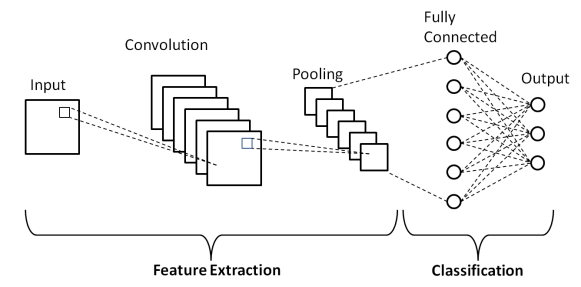
\includegraphics[width=.5\textwidth,height=.7\textheight,keepaspectratio]{tex/images/cnn.jpg}}
    \caption{CNN for fully connected network}
    \label{fig:my_label}
  





The fully connected network is almost similar to how neurons are arranged in a typical neural network.
Each node in a layer is connected directly to every node in both previous and in front layer.

One of the largest limitations of the traditional Neural Network is the fact that they tend to have a hard time 
with computational complexity that is required to process image data, hence the use of CNN becomes vital. \cite{o2015introduction}
As CNNs have become deeper and wider, problems of overfitting have been posed, primarily because of the
Dataset constraints, which are counterproductive to network generalization. For the avoidance of over-fitting,
One way is to alter the design of neural networks by adding dropout layers for example.


\subsection{Transfer Learning}
Transfer learning from a pre-trained network was used.
Transfer learning refers to an improved learning in a new task from a previously trained network. 
Transfer learning is machine learning with an additional source of information
apart from the standard training data: knowledge from one or more related tasks.\cite{torrey2010transfer}

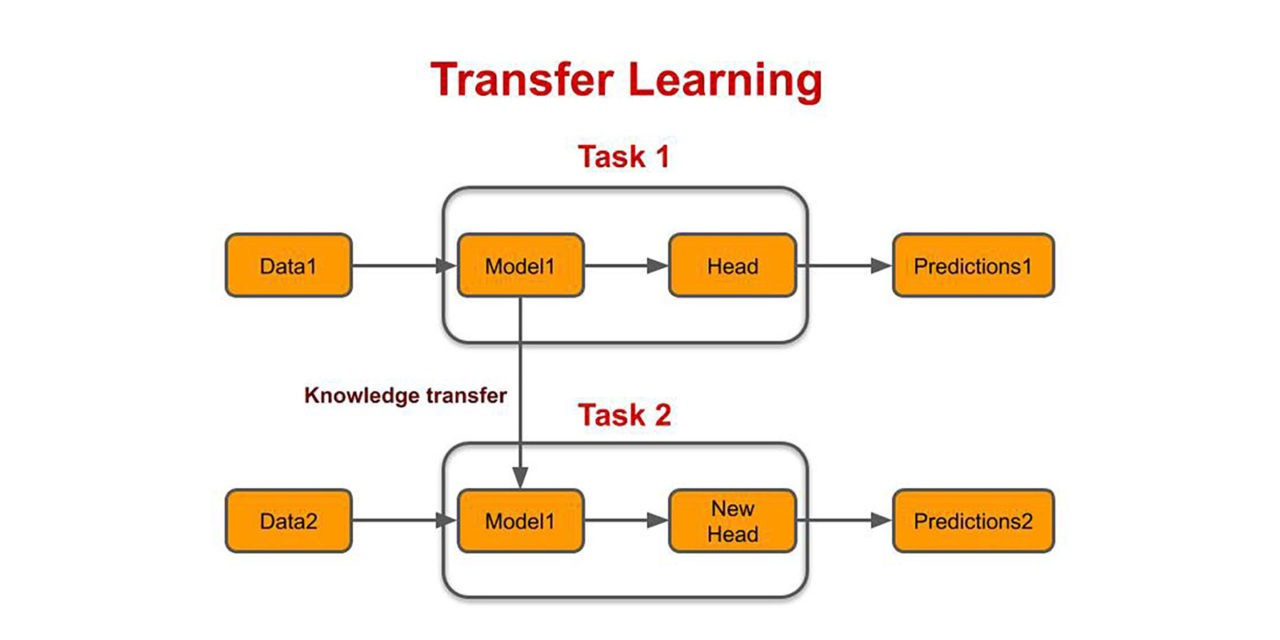
\includegraphics[width=.6\textwidth,height=.7\textheight,keepaspectratio]{tex/images/Transfer.jpeg}
\caption{Transfer Learning Model.}
\vspace{5mm}.


Thanks to this method, there is no need to re-train the entire model and as a result what is left is to work on the final classification part.
The InceptionV3 model is an architecture of convolutional networks. It is considered as one of the most accurate models for image classification. It was originally created by the Google Brain team.\cite{hussain2018study}
A transfer learning-based methodology is proposed in this paper that uses the
Pre-trained model for InceptionV3 to identify people who do not wear
Mask for the ears. The last layer of InceptionV3 is removed for this work and is tuned by adding 5 additional layers to the network. 
The 5 added layers are an
A typical pooling layer with a pool size equal to 5 x 5 was followed by a flattening layer,
A dense layer of 128 neurons with the activation and dropout feature of ReLU
A 0.5 rate, and finally a significant dense layer of two neurons and softmax. To classify if a person is wearing a mask, the activation feature is added. Sinno and Qiang \cite{pan2009survey}
in their paper have categorized Tansfer Learning techniques into three:
\begin{itemize}
    \item What transfer,
    \item How to transfer it and
    \item When to transfer it.
\end{itemize}

“What to transfer” asks which part of expertise can
be transferred throughout domain names or tasks. Some expertise is
precise for character domain names or tasks, and a few expertise
can be not unusual place among special domain names such that they may
assist enhance overall performance for the goal area or task. "How to transfer" is a product of which expertise may be transferred, learning
algorithms want to be advanced to switch the expertise. "When to transfer" then address the issue that asks wherein situations, transferring
abilities need to be done. Likewise, we're inquisitive about knowing
wherein situations, understanding need to now no longer be transferred


\subsection{Variational Autoencoder}

 It is a given fact that Deep Learning models has been exceedingly successful at learning data such as images, audio, and so on. However, it also has its limitations
 or challenges. Some of the challenges being biasedness when it comes to various things such as, but not limited to; skin color, gender, angle, etc. 
 Machine learning systems are increasingly making our day-to-day decisions that impact us daily as individual and also as a society. The development of an unbiased AI system
 like the one we have created is of paramount importance to limiting unintended side effects. \cite{amini2019uncovering} \vspace{5mm}.
 
 Autoencoders are trained to reconstruct the input data. Taking images as an input data in our case.
 Autoencoders are divided into two components, Encoders and Decoders.
 \item Encoder: a number of layers that are fully connected convolutional. They take he input and compress it down to very small representation
 to create what we call a bottleneck. 
 \item Decoded: A reconstruction from the bottleneck that gives the input of fully connected Convolution.
Variational Autoencoders provide a way to debias the image set, removing any bias towards variations in face positions, angle, and race.


A Variational Autoencoder (VAE) is an encoder that has a training that is regularised to avoid over-fitting and ensure that the 
latent space thus has good aspects that allow generative process.  

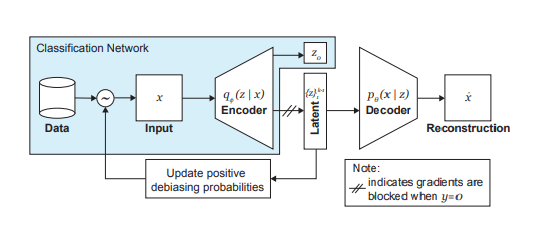
\includegraphics[width=.6\textwidth,height=.7\textheight,keepaspectratio]{tex/images/vae.png}
\caption{Debiasing Variational Autoencoder.}

To minimise the biasedness of our dataset, we train a VAE model to learn the latend structure that takes our dataset and debiases them with respect to facial features.


\subsection{TensorFlow}
A widely used Machine Learning (ML) task program is TensorFlow (TF). It is generally adopted, as it offers an interface to express the models' typical ML algorithms and executable code. Models generated in TensorFlow  can be transported with devices ranging from heterogeneous systems with little to no shift.
From cell phones to servers that are distributed. 
\vspace{5mm}.

TensorFlow  has been developed by and is maintained by Google and is used internally within the organization for the purposes of Machine Learning.
In our system, Tensorflow is thus a preferred library that we used.TensorFlow could be a machine learning framework that works at expansive scale and in heterogeneous situations. TensorFlow employments dataflow charts to speak to computation, shared state, and the operations that change that state. It maps the hubs of a dataflow chart over numerous machines in a cluster, and inside a machine over different computational gadgets, counting multicore CPUs, generalpurpose GPUs, and custom-designed ASICs known as Tensor Processing Units (TPUs).

\begin{lstlisting}
import tensorflow as tf

b = tf.Variable(tf.zeros([100]))                        #100-d vector, init to zeros
W = tf.Variable(tf.random_uniform([784,100],-1,1))      #784x100 matrix
x = tf.placeholder(name="x")                            #Placeholder for input
relu = tf.nn.relu(tf.matmul(W,x) + b)                   #Relu(Wx+b)
C = [...]                                               #Cost computed as a function of Relu


s = tf.Session()
for step in xrange(0,10):
    inout = ...construct 100-D input array ...
    result = s.run(C, feed_dict={x: input})
    print step, result
\end{lstlisting}
The above code is an example of a Tensorflow code fragement. \cite{abadi2016tensorflow}.
The above code is to bring a general understanding of Tensorflow in a session. In our system, Tensorflow is used together with keras during the training of our model.

\subsection{OpenCV}
OpenCV (Open Source Computer Vision) is short for Open Source Computer vision. OpenCV is an open source image and video processing library that was originally introduced by Intel more than a decade ago.  \cite{culjak2012brief}
Computer vision is one of the paramount disciplines in programming a computer to gain visualisation and understanding of images as well as videos, in simple terms, it is allowing the computer to see.
\vspace{5mm}.

The goal of Intel team in 1999 when they launched OpenCV was to offer a library that would be useful in programming functions that is an optimal code available for free.OpenCV offers progressed video investigation on video sequences as well. Other than essential operations such as reading/viewing/writing video arrangements, extricating person outlines etc. a ordinary two errands are the closer view extraction and question following.It is basic to note in spite of the fact that that in arrange for OpenCV to open a indicated video record, the comparing codec must be introduced on the computer. Other than, there's a plausibility to examined specifically the video stream of a associated camera \cite{culjak2012brief}.
The basic image processing and higher level computer vision algorithms are contained in the CV component.
We have used an OpenCV for the detection of real-live movement on the web-cam to be able to detect the movement of the face as well as the mask. The use of this library is both easy to use and is relevant in this system. 

In our system we started by importing the CV2 and we use the CV2.VideoCapture to use the camera. Furthermore, we use CascadeClassifier to load the XML file 'haarcascade frontalface default.xml'

cv2.resize is then used to resize the image to speed up the detection. cv2.rectangle are used to draw rectangles across the faces. cv2.show is to go live and display the webcam.





